\documentclass[tikz,border=10pt]{standalone}
\usepackage[scaled=0.95]{helvet}
\renewcommand{\familydefault}{\sfdefault}
\usepackage{tikz}
\usetikzlibrary{arrows.meta,positioning,shapes.geometric}
\definecolor{TEJNavy}{HTML}{1E2B55}
\definecolor{TEJBlue}{HTML}{1769AA}
\definecolor{TEJGreen}{HTML}{2B7A53}
\definecolor{TEJGold}{HTML}{D49B19}
\definecolor{TEJLight}{HTML}{EEF6F8}
\begin{document}
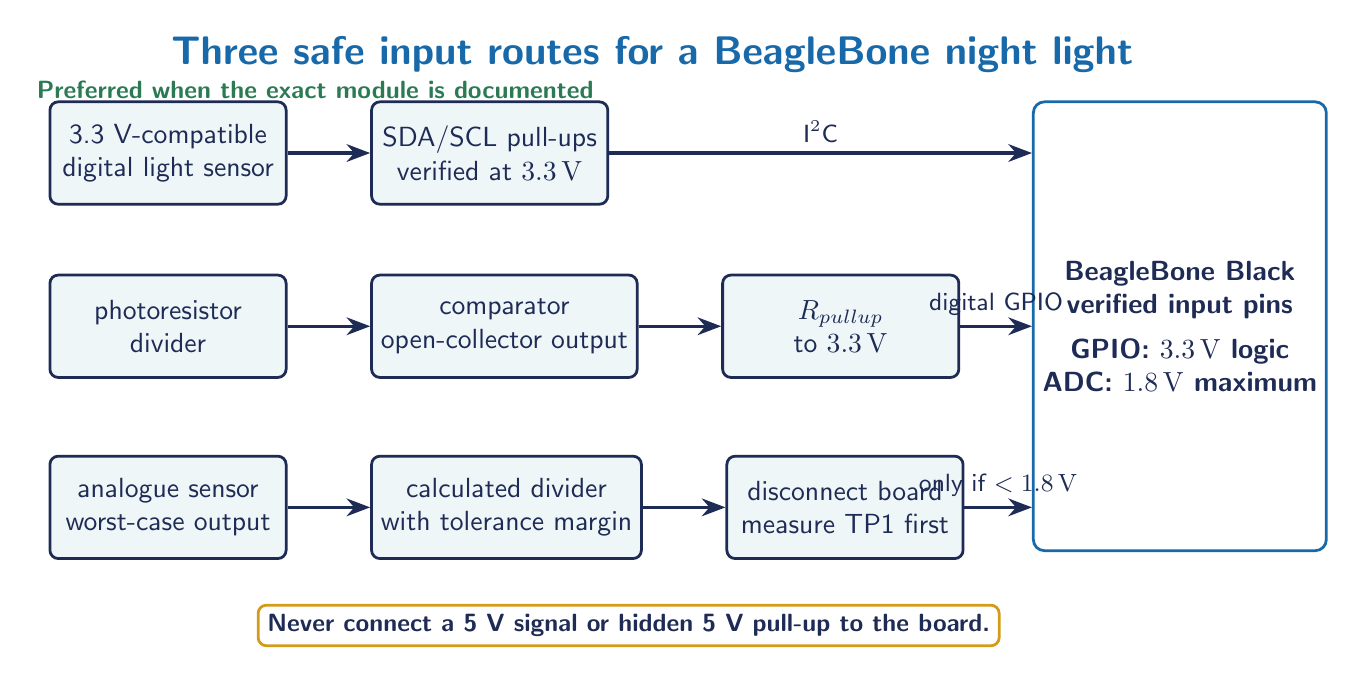
\begin{tikzpicture}[
  font=\sffamily,
  text=TEJNavy,
  line width=1.0pt,
  block/.style={draw=TEJNavy,rounded corners=3pt,fill=TEJLight,minimum width=3.0cm,minimum height=1.3cm,align=center},
  board/.style={draw=TEJBlue,rounded corners=4pt,fill=white,minimum width=3.3cm,minimum height=5.7cm,align=center,font=\bfseries},
  arrow/.style={-{Stealth[length=3mm]},draw=TEJNavy,line width=1.2pt}
]
  \node[font=\bfseries\Large,text=TEJBlue] at (8.3,7.0)
    {Three safe input routes for a BeagleBone night light};

  \node[board] (bbb) at (15.0,3.55) {BeagleBone Black\\verified input pins\\[4pt]
    GPIO: $3.3\,\mathrm{V}$ logic\\ADC: $1.8\,\mathrm{V}$ maximum};

  \node[block] (i2c) at (2.15,5.75) {3.3 V-compatible\\digital light sensor};
  \node[block,right=1.05cm of i2c] (pullups) {SDA/SCL pull-ups\\verified at $3.3\,\mathrm{V}$};
  \draw[arrow] (i2c) -- (pullups);
  \draw[arrow] (pullups.east) -- node[above,font=\small]{I$^2$C} (bbb.west |- pullups.east);
  \node[anchor=west,text=TEJGreen,font=\bfseries\small] at (0.35,6.55) {Preferred when the exact module is documented};

  \node[block] (divider) at (2.15,3.55) {photoresistor\\divider};
  \node[block,right=1.05cm of divider] (comp) {comparator\\open-collector output};
  \node[block,right=1.05cm of comp] (pu33) {$R_{pullup}$\\to $3.3\,\mathrm{V}$};
  \draw[arrow] (divider) -- (comp);
  \draw[arrow] (comp) -- (pu33);
  \draw[arrow] (pu33.east) -- node[above,font=\small]{digital GPIO} (bbb.west |- pu33.east);

  \node[block] (analog) at (2.15,1.25) {analogue sensor\\worst-case output};
  \node[block,right=1.05cm of analog] (scale) {calculated divider\\with tolerance margin};
  \node[block,right=1.05cm of scale] (meter) {disconnect board\\measure TP1 first};
  \draw[arrow] (analog) -- (scale);
  \draw[arrow] (scale) -- (meter);
  \draw[arrow] (meter.east) -- node[above,font=\small]{only if $<1.8\,\mathrm{V}$} (bbb.west |- meter.east);

  \node[draw=TEJGold,fill=white,rounded corners=3pt,align=center,font=\bfseries\small]
    at (8.0,-0.25) {Never connect a 5 V signal or hidden 5 V pull-up to the board.};
\end{tikzpicture}
\end{document}
